% Recursive plans for right_split and corner_split, for Section 2.2.4.
% Redrawn from upstream's figure 2.13, with the names in their Python spelling.
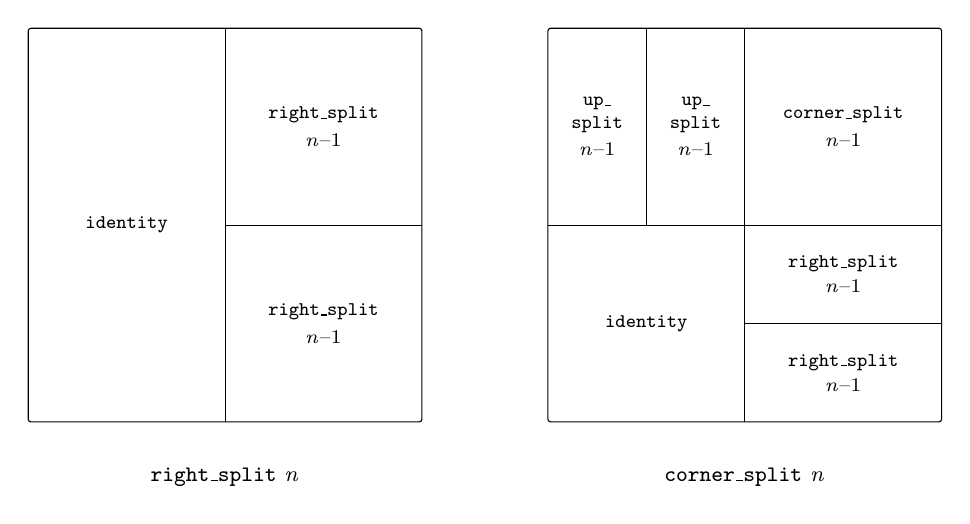
\begin{tikzpicture}[
  x = 1mm, y = -1mm,
  % No draw: the panels are the rectangles below, the labels sit inside them.
  cell/.style    = {align=center, font=\scriptsize},
  caption/.style = {font=\footnotesize},
]

% --- right_split n : identity on the left, two smaller splits stacked right
\draw[rounded corners=1pt] (0, 0) rectangle (50, 50);
\draw (25, 0) -- (25, 50);
\draw (25, 25) -- (50, 25);
\node[cell] at (12.5, 25) {\texttt{identity}};
\node[cell] at (37.5, 12.5) {\texttt{right\_split}\\[2pt]\textit{n}--1};
\node[cell] at (37.5, 37.5) {\texttt{right\_split}\\[2pt]\textit{n}--1};
\node[caption] at (25, 57) {\texttt{right\_split} \textit{n}};

% --- corner_split n
\begin{scope}[xshift=66mm]
\draw[rounded corners=1pt] (0, 0) rectangle (50, 50);
\draw (25, 0) -- (25, 50);
\draw (0, 25) -- (50, 25);
\draw (12.5, 0) -- (12.5, 25);
\draw (25, 37.5) -- (50, 37.5);
\node[cell] at (6.25, 12.5) {\texttt{up\_}\\\texttt{split}\\[2pt]\textit{n}--1};
\node[cell] at (18.75, 12.5) {\texttt{up\_}\\\texttt{split}\\[2pt]\textit{n}--1};
\node[cell] at (37.5, 12.5) {\texttt{corner\_split}\\[2pt]\textit{n}--1};
\node[cell] at (12.5, 37.5) {\texttt{identity}};
\node[cell] at (37.5, 31.25) {\texttt{right\_split}\\[1pt]\textit{n}--1};
\node[cell] at (37.5, 43.75) {\texttt{right\_split}\\[1pt]\textit{n}--1};
\node[caption] at (25, 57) {\texttt{corner\_split} \textit{n}};
\end{scope}

\end{tikzpicture}
